\documentclass[a4paper,12pt,ngerman]{scrartcl}

% Language
\usepackage{polyglossia}
\setmainlanguage{german}

% Grafiken
\usepackage{graphicx}

% Make \today print in format "NN<st|nd|rd|th> MM YYYY"
\usepackage{isodate}
\origdate

\linespread{1.15}

\usepackage{pdfpages}

% Titel anders formatieren mit: Command, Format, Label, Sep, Before-Code
\usepackage{titlesec}
\titleformat{\section}{\sffamily\Large\bfseries}{}{0pt}{}
\titleformat{\subsection}{\sffamily\large\bfseries}{}{0pt}{}

% Own pagestyle (header and footer)
\usepackage{fancyhdr}
\fancyhf{} % Clear header and footer content
\fancyhead[L]{{\small \textsf{WS 14/15, Informationsvisualisierung}}}
\fancyhead[C]{{\small \textsf{Übung 6}}}
\fancyhead[R]{{\small \textsf{\today}}}
\fancyfoot[C]{\thepage}

% Text in quotes
% Usage: \enquote{To be or not to be.}
\usepackage{csquotes}

% Subliminal refinements towards typographical perfection
\usepackage{microtype}

% Footnotes in section
\usepackage[stable]{footmisc}

\usepackage{hyperref}

% Better refs with \cref{}
\usepackage[capitalize,noabbrev]{cleveref}

% Borders
\usepackage[paper=a4paper,left=20mm,right=20mm,top=30mm,bottom=30mm]{geometry}

\usepackage{placeins}

\begin{document}
\pagestyle{fancy} % Activate own pagestyle

\section{Aufgabe 6.1 | Konzeptionierung einer interaktiven Visualisierung}
Wir haben uns dafür entschieden, den Datensatz über das Trinkverhalten von Homer Simpson zu visualisieren.

\subsection{Aufgabe 6.1a | Beschreibung des Anwendungsgebiets und der Daten}
Datentyp: diskret, Datenstruktur: temporal, multivariat

Einem Datum werden mehrere Werte zugeordnet, diese sind in erster Linie die Mengen der Flüssigkeiten, die zugenommen wurden, sowie die daraus resultierenden Zucker-, Koffein- und Alkoholmengen. In der zeitlichen Dimension müssen zusätzlich bestimmte Zeitpunkte hervorgehoben werden. In der Dimension der Zuckerwerte (Koffein-/Alkoholwerte) müssen diese in Relation zu einem festen Wert gesetzt werden, der empfohlenen Maximaldosis. Außerdem sind verschiedene Granularitätsstufen gegeben, die Ergebnisse sind pro Tag, Monat oder Jahr anzugeben.

\subsection{Aufgabe 6.1b | Zielgruppenanalysse}
Die Visualisierung wird vor allem medizinischem Fachpersonal (Ärzte, Psychotherapeuten, ...) dienen. Sie haben meist wenig Zeit, sich auf einen Patienten einzustellen, weshalb eine effiziente Visualisierung der wichtigen Daten eine große Erleichterung darstellen kann. In der Branche spielen fast alle Arten von Visualisierungen eine Rolle, häufig handelt es sich um diskrete Zahlenwerte, die mit einem Zeitpunkt (oder mehreren Zeitpunkten) in Verbindung gebracht werden oder 3D-Abbildungen von Körperteilen.

\subsection{Aufgabe 6.1c | Zweck der Visualisierung}
Die Visualisierung soll dem Betrachter zunächst einen Überblick über den Gesundheitszustand des Patienten (Homer Simpson) geben und auf mögliche Probleme aufmerksam machen. Zu solch kritischen Bereichen gibt die Visualisierung auch die Möglichkeit, sich im Detail über die Zunahme verschiedener Getränke bzw. deren Inhaltsstoffe (Zucker, Koffein, Alkohol) zu informieren.

\subsection{Aufgabe 6.1d | Konzepterstellung}
Die Basis der Visualisierung bildet ein Liniendiagramm, auf dem auf der x-Achse die Zeit und auf der y-Achse die Mengen (in ml) der verschiedenen zugenommenen Flüssigkeiten (Wasser, Saft, Milch, Cola, Kaffee, Bier) aufgetragen werden. Die Zugehörigkeit der Linien zur bestimmten Flüssigkeit wird durch Farbe und Beschriftung dargestellt.

Zunächst erfolgt die Darstellung durch jährlich konsolidierte Daten, um einen Überblick über das gesamte bisherige Leben des Patienten zu geben. Es ist möglich, einen Zeitraum daraus auszuwählen, um eine monatliche oder im weiteren Schritt eine tägliche Aufschlüsselung der Daten zu erhalten.

Die besonderen Zeitpunkte werden durch vertikale Striche über die Gesamthöhe der Visualisierung (Diagramm und Zusatzinformationen, s.u) markiert.

Unterhalb des Diagramms befinden sich, aufteilt in drei Zeilen, Informationen zu den Zucker-, Koffein- und Alkoholzunahmen. Um einen Überblick über bedenkliche Werte zu erhalten, wurde eine Kodierung in drei Farben eingeführt. Grün bedeutet, dass der Maximalwert pro Tag im jeweiligen Zeitraum an keinem überschritten wurde. Gelb bedeutet, dass der Maximalwert an mindestens einem Tag im betrachteten Zeittraum überschritten wurde. Rot bedeutet, dass der Maximalwert an mindestens $x$ Tagen überschritten wurde. Dieser Wert $x$ kann durch den Betrachter über einen Schieberegler eingestellt werden (Standardwert: 50\% der Tage).

Um zu erfahren, wie sich z.B. hohe Zucker- oder Koffeinwerte zusammensetzen, können zu jedem Zeitraum (Tag, Monat oder Jahr) durch Klick auf die entsprechende Zeile ein weiteres Diagramm hervorgerufen werden. Es zeigt welchen Anteil die verschiedenen Flüssigkeiten am Gesamtwert haben, daran ist also z.B. abzulesen, ob ein hoher Zuckerwert von zu viel Zucker im Kaffee oder einem hohen Saft- oder Colagenuss entstanden ist.
\\\\
Vorteile dieser Visualisierung: schneller Überblick, Detailinformationen durch ein bis zwei Klicks abfragbar, angemessene Informationsmenge pro Darstellung (nicht zu viel Information auf einmal), Warnungen bei übermäßigem Konsum, Einstellung auf Patienten möglich
\\\\
Nachteile, Verbesserungs- und Erweiterungsmöglichkeiten:

\subsection{Aufgabe 6.1e | Fake-Screenshots, Mockup}
Die Fake-Screenshots bzw. das Mockup finden Sie auf der nächsten Seite.

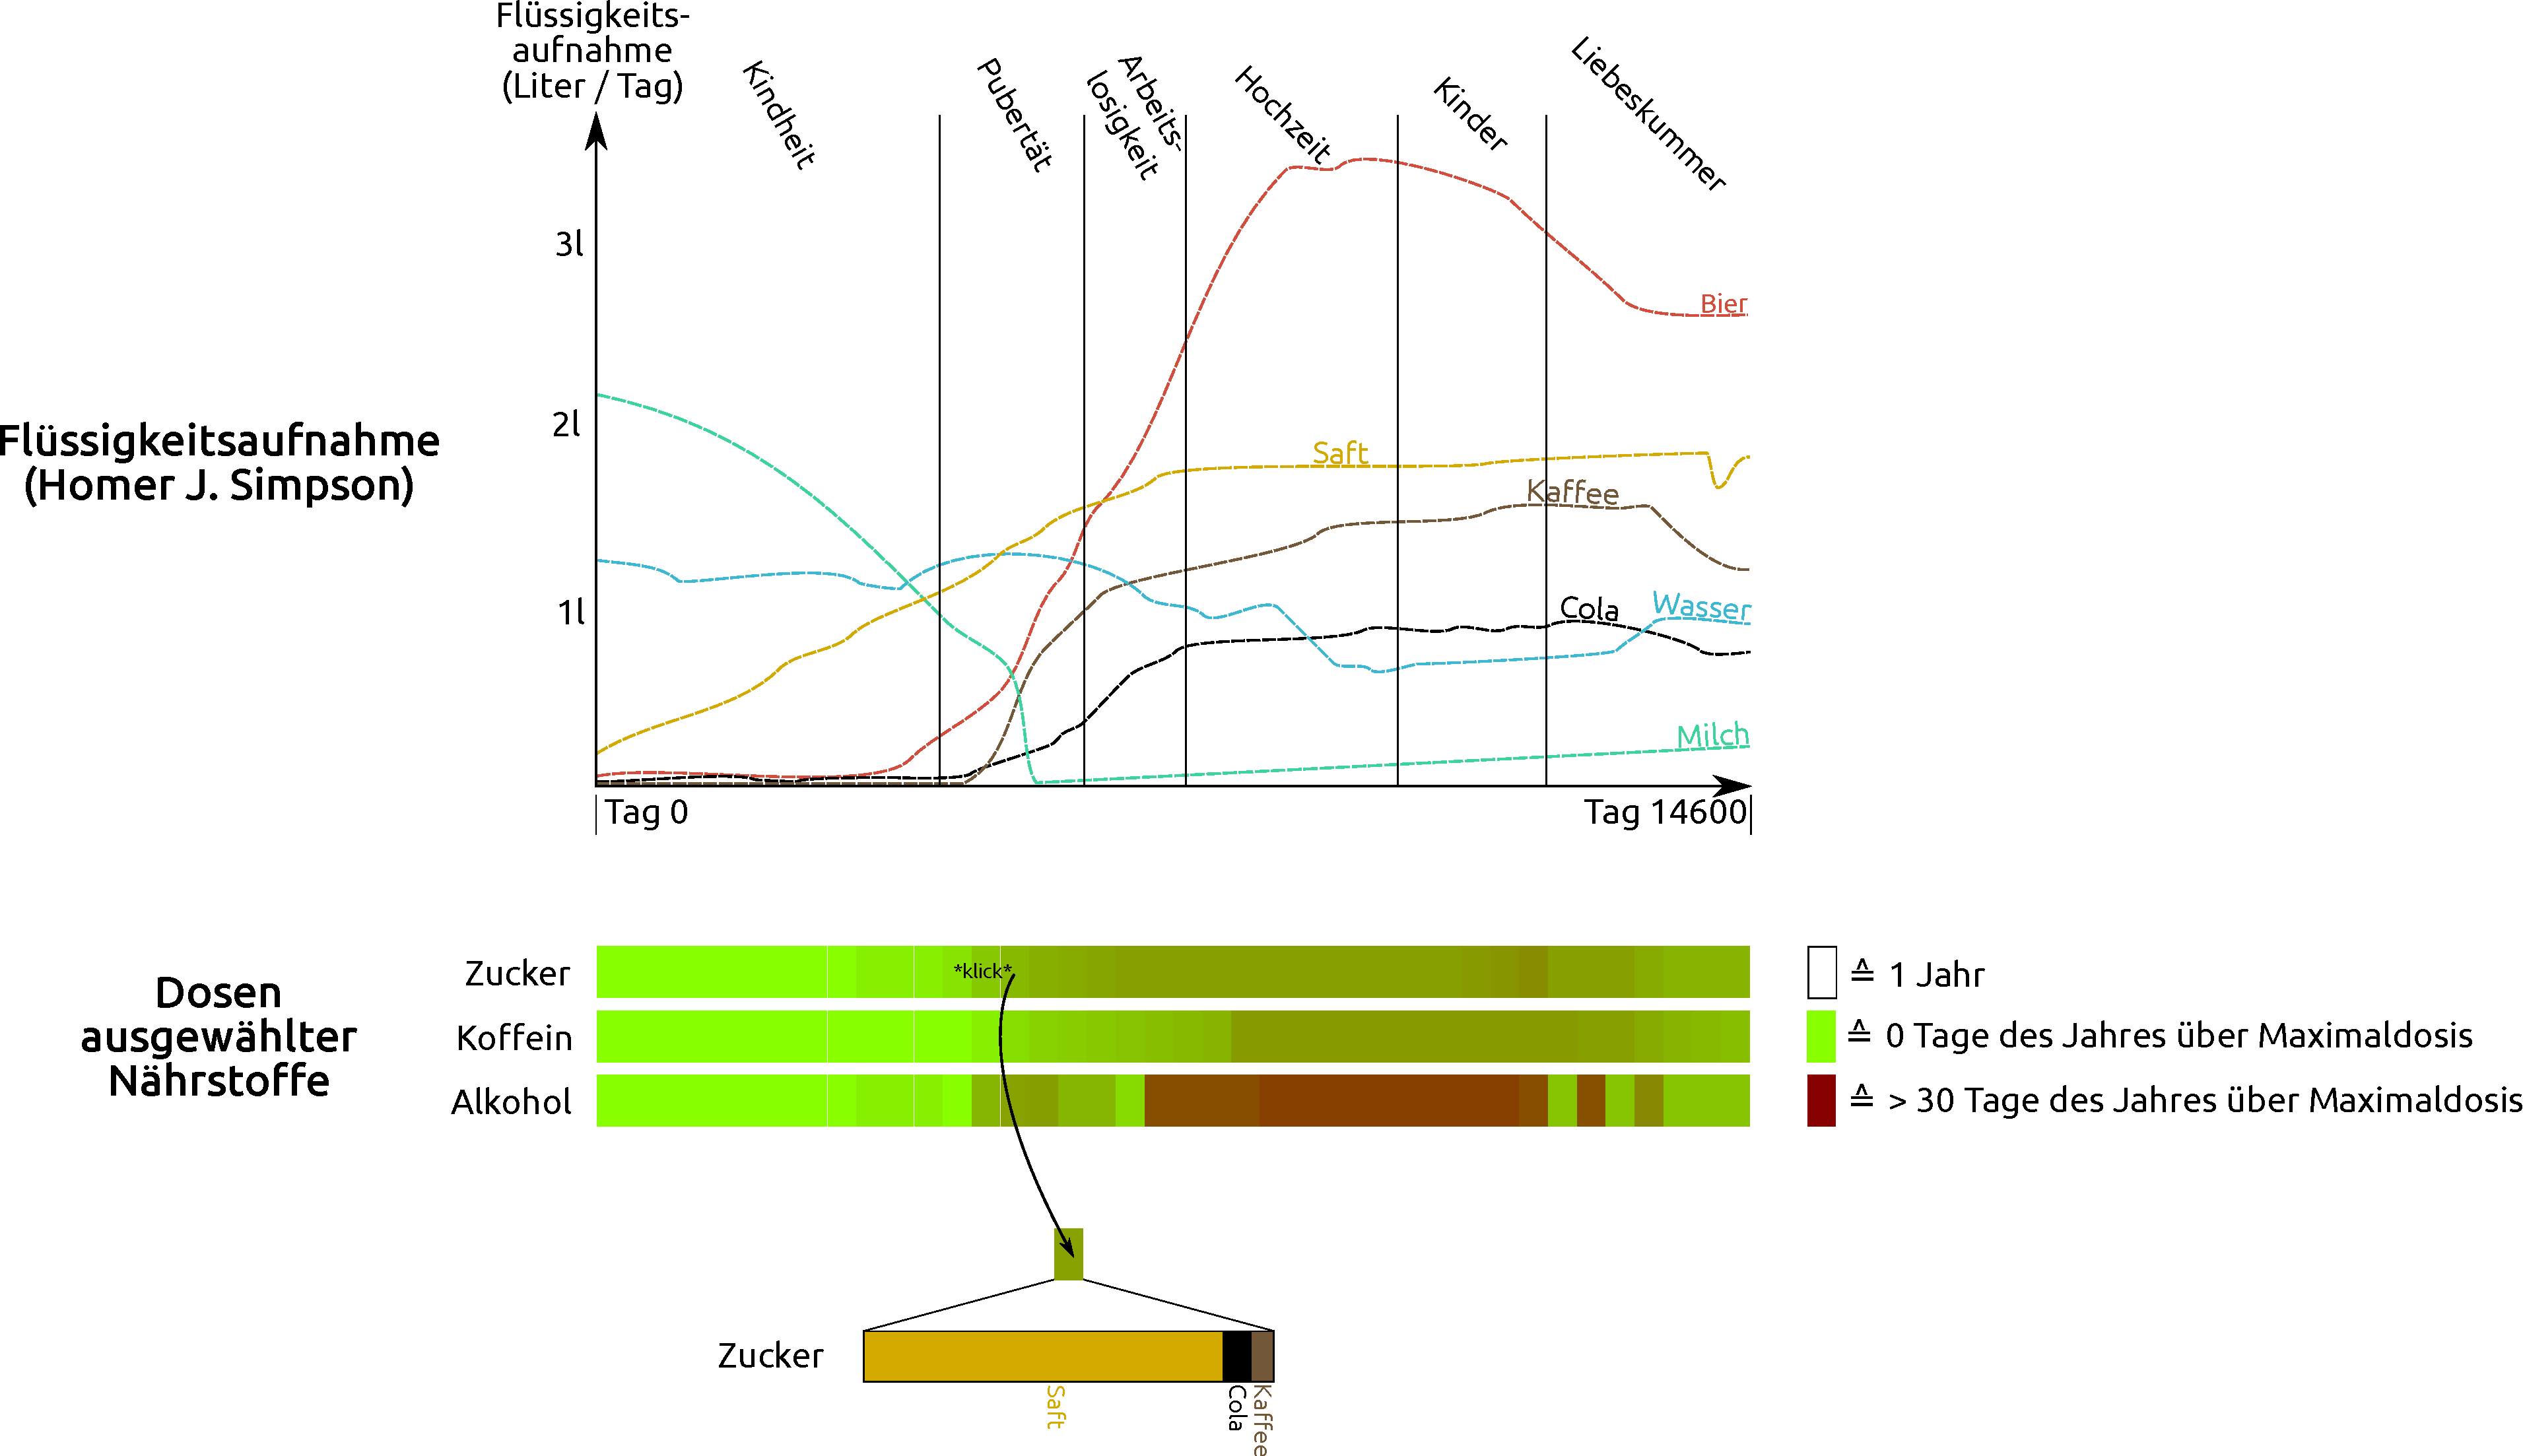
\includepdf[landscape=true,pages={-}]{Overview.pdf}

\end{document}
